\subsection{Radio Frequency Module Reception Test} % (fold)
\label{cha:radio_frequency_module_reception_test}
To test how the \gls{rf}-modules works, a test has been devised. 
The purpose of this test is to test the range of the \gls{rf}-modules with different antennas and across different ranges. 
The test will use the RadioHead library as described in \myref[name]{subsubsec:RadioHead}. 
Built into RadioHead is a \gls{crc} check, this ensures the integrity of the message received. 

\subsubsection*{Test setup}
We will test the following three different antenna configurations: 
\begin{description}[labelindent=\parindent, labelwidth=\widthof{\bfseries 17.3 cm}, align=parright]
    \item[0 cm] No external antenna
    \item[12 cm] An arbitrary antenna length
    \item[17.3 cm] A quarter-monopole antenna (at 433 MHz using \myref{QMA})  
\end{description}
Each will be used on both the receiver and the transmitter. 
This yields six combinations which will be tested. 
Many receivers can receive the same message, therefore all receivers can be tested at the same time. 
We have tested with distances from 2 metres to 28 metres, except for the test with a 0 cm antenna on the transmitter where a high package loss was occurring even at ranges of 14 metres. 

The transmitter was placed on a table 1 meter above the ground.
The LED connected to the Arduino was used as a visual aid blinking every time a package was sent
This has no real influence on the test and was used as a convenience for those who tested.

The receivers were placed on a table 1 meter above the ground, each 15 cm away from the others.
The LED on those devices was set to blink whenever a package was received.

First the transmitters and receivers were 2 meters from each other then a test with 100 packets containing 16 bytes was sent, the contents of a single message was the index of the packages being sent. 
The receivers counted the messages received and wrote the final result to the computer over USB. 
This was repeated every 2 metres. 
The code run on the Arduinos can be found in \myref{app:PkgLossRxCode} and \myref{app:PkgLossTxCode}.  

% \begin{figure}[p]
% \centering
% 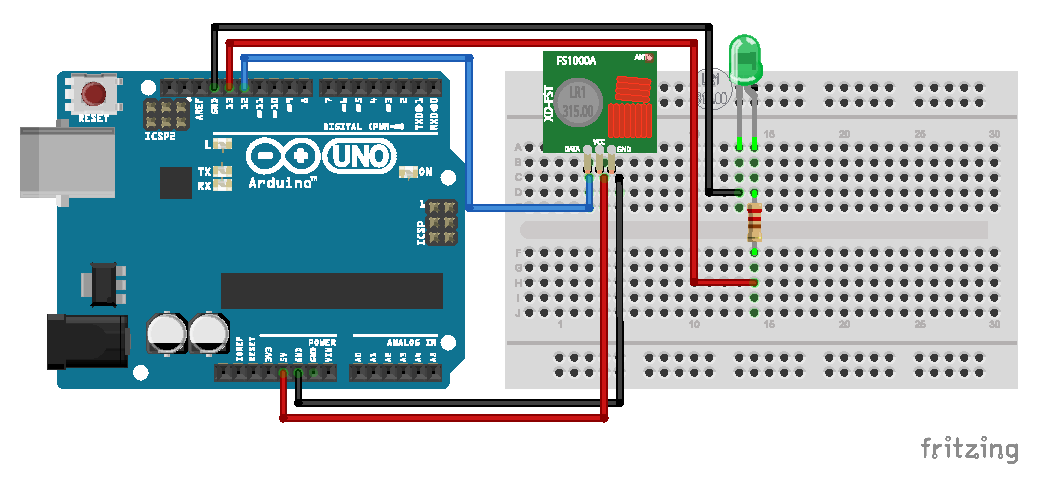
\includegraphics[width=\linewidth]{Figures/Fritzing/Transmitter.pdf} 
% \caption{Graphical circuit diagram of an Arduino with a transmitter.}
% \label{fig:Transmitter}   
% \end{figure}

% \begin{figure}[p]
% \centering
% 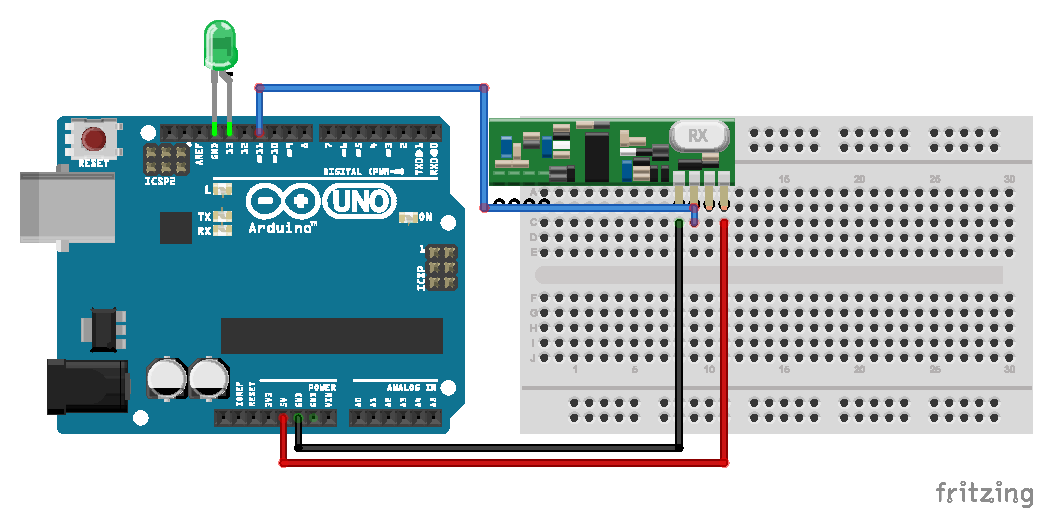
\includegraphics[width=\linewidth]{Figures/Fritzing/Receiver.pdf} 
% \caption{Graphical circuit diagram of an Arduino with a receiver.}
% \label{fig:Receiver}   
% \end{figure}

\subsubsection*{Results}
The results of the test have been plotted in three separate graphs, this approach has been chosen so that it is easier to focus on the difference in antenna length on the receiving end.
\figur{Graphs/0cm_ant.pdf}{0.9}{Package loss percentage at different distances with no antenna on the transmitter.}{0cm_ant}
\figur{Graphs/12cm_ant.pdf}{0.9}{Package loss percentage at different distances with 12 cm antenna on the transmitter.}{12cm_ant}
\figur{Graphs/17cm_ant.pdf}{0.9}{Package loss percentage at different distances with 17.3 cm antenna on the transmitter.}{17cm_ant}


\subsubsection*{Analysis}
Across all three graphs, the plots representing the receiver with an antenna length of 17.3 cm shows the lowest package loss. 
The only place where the results are difficult to distinguish from each other is in the graph where the transmitter has an antenna length of 17.3 cm (see \myref{fig:17cm_ant}); here all the different lengths of receiver antennas demonstrates a low package loss percentage compared to the other graphs.
This could show that the transmitter and its antenna has a significant impact on the reliability of the transmission of data.
In fact, the package loss of the receiver not fitted with any external antenna is indistinguishable from the receiver with 17.3 cm external antenna.

Furthermore, the three graphs indicate that the antenna length of 12 cm on the receiver does not help the reception.
On the contrary, it worsens the ability to receive messages.
But an antenna length of 12 cm does not decrease the reliability as much when it is fitted on the transmitter (see \myref{fig:12cm_ant}), this could be due to an error in the test setup, or just the fact that the transmitter is able to send a much stronger signal as soon as an external antenna is introduced.

\begin{table}[ht]
\centering
\begin{tabular}{r r r r r}    \toprule
 && \multicolumn{3}{c}{\textbf{Rx module}}\\
 && \textbf{0 cm}    & \textbf{12 cm}    & \textbf{17.3 cm}  \\\midrule
\multirow{3}{*}{\textbf{Tx module}}  &\textbf{0 cm} & 55.00 \%   & 60.86 \% & 21.68 \% \\ 
 &\textbf{12 cm} & 7.14 \% & 31.71 \% & 1.21 \%  \\ 
 &\textbf{17.3 cm} & 0.93 \% & 12.71 \% & 1.29 \%  \\\bottomrule
 \hline
\end{tabular} 
\caption{Table of average package-loss in percentage for varying lengths of antennas.}
\label{tbl:packageloss}
\end{table}

\bigskip
\noindent
In \myref{fig:0cm_ant}, it is indicated that whether the transmitter has an external antenna affects the reliability of the transmitted signal as we can observe that the lack of an external antenna on the transmitter produces a high package loss percentage on the receiving end.

An average of the results from the graphs has been calculated and omitted into a table which can be found on \myref{tbl:packageloss}. 
This shows that using antennas of the length 17.3 cm will cause the transmissions to have a package loss of \textasciitilde1~\%.
The results will be further concluded upon later.

\paragraph{What Causes the Package Loss?}\label{par:wctpl}\hfill \\
A small sub-test has been made to explore if when a package is lost for one device, is the same package lost amongst all other devices.
This is done by having one Arduino with a transmitter, with an antenna length of 17.3 cm, transmitting the numbers from zero to 999, and having three Arduinos with an antenna length of 17.3 cm receiving the data. 
If a package is missed for one Arduino is it then the same number which is missed across all Arduinos.
This will help discover if the problem of package loss is connected to the receivers or to the transmitters.

The results were that one device missed 14 transmissions, while the other two devices received all the transmissions.
For the rest of this paper, it is assumed that whenever a transmission is not received it is due to the receiver, and thus not because of a fault on the transmitter's side.
But external factors can still play a role and cause package loss, this will be ignored.

\subsubsection*{Sources of error}
There are many possible source of error within the test with antenna lengths, which all needs to be considered to conclude upon the results.
The most significant and the ones that are most likely to occur are as follows:
\begin{description}[labelindent=\parindent]
    \item[Objects placed in the way of the signal] \hfill \\
    In order for the results to represent real world scenarios, one could test the package loss with different objects between the transmitter and receiver. 
    E.g. humans, construction objects, furniture.
    But as this test was looking for quantitative data the results were gathered with no object in the way of the signal, so that the conditions and data of the tests would be comparable.
    \item[Signal interference] \hfill \\
    This category of errors is one of the most remarkable since any form of signal interference could invalidate the data and even produce false positives.
    To avoid as much signal interference as possible, the test was conducted in a basement with thick concrete walls, and equipment that uses the same frequency e.i. 433 MHz was kept away from the test setup.
    \item[Inaccuracy in distance and antenna length] \hfill \\
    The margin of error on the measured distance between the probes is within a few centimetres, and since each probing was done in increments of two meters it is to be considered insignificant.
    But, the tolerable margin of error when considering the length of the antennas is much smaller than two centimetres.
    Such varying in antenna length would have drastic consequences due to the antenna length's dependence upon the wavelength of the signal.
    The antennas used in this test were measured to specific lengths of 12 and 17.3 cm.
    It is noteworthy that the internal antennas of both the transmitter and receiver modules may affect the results.
    \item[Difference in \acrshort{rf}-modules] \hfill \\
    To be able to compare the results of the different antennas, one must assure that the difference in results is not induced by differences in the \gls{rf}-modules.
    But, by testing all the used \gls{rf}-modules as done in \myref[name]{cha:radio_frequency_module_difference_test}, this source of error is to be considered close to non-existent, since all the \gls{rf}-modules used in this test, showed less package loss than 2 \%.
    This source of error is hereby deemed insignificant for the results of this test.
\end{description}

\subsubsection*{Conclusion}
The 17.3 cm antenna on the transmitter has the biggest impact on the package loss rate.
This is in line with the theory of using a quarter-wave monopole antenna.
This implies that using a 17.3 cm antenna on both the receiver and transmitter will benefit the connection, both for range, and reliability.
The only downside is that the size will increase.
But, this trade-off is worth it for the project as a whole.
The amount of package loss still occurring with the 17.3 cm antennas shows that it is uncertain that a message being transmitted will be received.
For the project, this means that the technique used to control the communication between the Arduinos needs to take into account that a transmission might not be received.
% chapter radio_frequency_module_reception_test (end) 
